\documentclass[crop=false,fleqn]{standalone}
\usepackage{../../../globle-preamble}

\begin{document}
    \textbf{Find the domain and range of the funtion $g$ and sketch graph of $g$.}

    $$ g(x) = \sqrt{x+1} $$

    \vspace{1em}
    Domain of $g(x)$ = $[-1,+\infty)$

    Range of $g(x)$ = $[0,+\infty)$
    \vspace{1em}

    \begin{center}
        \begin{tabular}{ |c|c|c|c|c|c|c| } 
            \hline
            $x$ & -1 & 0 & 1 & 2 & 3 & 4 \\ 
            \hline
            $g(x)$ & 0 & 1 & $\sqrt{2}$ & $\sqrt{3}$ & 2 & $\sqrt{5}$ \\
            \hline
        \end{tabular}
    \end{center}

    \begin{center}
        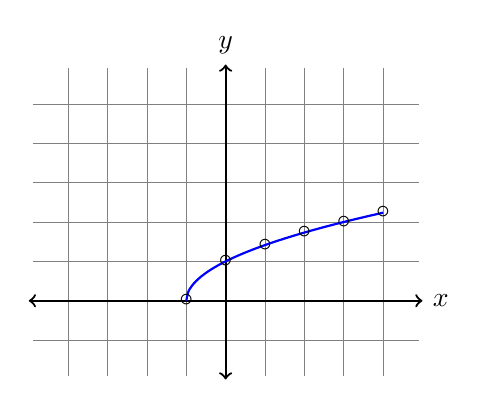
\begin{tikzpicture}[scale=0.5]
            \draw[step=1,gray,very thin] (-4.9,-1.9) grid (4.9,5.9);
            \draw[<->,thick] (-5, 0) -- (5, 0) node[right] {$x$};
            \draw[<->,thick] (0, -2) -- (0, 6) node[above] {$y$};
            
            \draw[domain=-1:4, samples=105, smooth, variable=\x, thick, blue]
                plot ({\x}, {sqrt(\x+1)});

            \foreach \Point in {(-1,0), (0,1), (1,1.414), (2,1.73), (3,2), (4,2.236)}{
                \node at \Point {$\circ$};
            }
        \end{tikzpicture}
    \end{center}
\end{document}
